\chapter[Concepção]{Concepção}

\section{Introdução}

O tratamento térmico é o conjunto de operações de aquecimento e resfriamento a que são submetidos materiais sob condições controladas, com o objetivo de alterar suas propriedades ou conferir-lhes características mecânicas e estruturais diferentes.

Os tratamentos mais usuais são o recozimento, a normalização, a têmpera, o revenido e o coalescimento. Esses tratamentos são influenciados por alguns fatores que são: o aquecimento, tempo de permanência em determinada temperatura, resfriamento e atmosfera de aquecimento, portanto cada tratamento específico necessita do controle desses fatores.

Portanto um forno de tratamento térmico é de fundamental importância para se realizar esses tratamentos, logo para que o tratamento seja satisfatório, o forno deve ser capaz de variar a temperatura e manter a temperatura de forma satisfatória, de acordo com o tratamento requerido, sem que a temperatura do ambiente externo seja elevado a condições insalubres.

\section{Justificativa}

Uma das atividades de grande importância na ciência dos materiais é o tratamento térmico, que de acordo com Tschiptschin é um ciclo de aquecimento e resfriamento realizado nos metais com o objetivo de alterar as suas propriedades físicas e mecânicas, sem mudar a forma do produto. O tratamento térmico acontece também inadvertidamente, como consequência de um processo de fabricação que cause aquecimento ou resfriamento no metal, como nos casos de soldagem e de forjamento. Esses tratamentos são utilizados em várias situações diferentes como na indústria para alterar características de fabricabilidade, como usinabilidade, estampabilidade ou restauração de ductilidade de metais, o meio acadêmico para o estudo das estruturas microcristalinas dos metais e sua influência nas propriedades do material, e no meio empreendedor como ferramenta para tratamento de vários produtos.

\section{Contextualização}

Um grupo de 14 pessoas de todas as engenharias (Aeroespacial, Automotiva, Eletrônica, Energia e Software) do campus foi montado visando o desenvolvimento de um forno para tratamentos térmicos, desde a teoria até o produto final. Para tal, diversas reuniões presenciais foram realizadas, bem como a utilização de ferramentas de comunicação online e de armazenamento e compartilhamento de arquivos.

A escolha do tema, bem como das características do forno foram motivadas pela necessidade de ampliar a capacidade da Universidade de Brasília (UnB) de realizar experimentos acerca de materiais. Na idealização do forno, considerou-se a têmpera como a forma de verificação do funcionamento do forno e o aço o material que será tratado. Pretende-se, após a fabricação do forno, disponibilizá-lo para a UnB.

\subsection{Proposta}

Visa-se, ao final do projeto, a fabricação de um forno que possa ser utilizado para o tratamento térmico dos mais diversos materiais, sem que sua superfície externa apresente temperaturas maiores que $60 \degree \text{C}$ e que seja capaz de elevar sua temperatura interna até $1200 \degree \text{C}$ de forma controlada. A progressão da temperatura interna poderá ser definida pelo usuário para atender à sua necessidade.

\section{Tecnologias Existentes}

O mercado de fornos para tratamentos térmicos possui uma grande variedade de modelos e fabricantes devido às diferentes aplicações e a importância desses processos na indústria como um todo. Para atender as diferentes aplicações há um grande número de variações nas especificações. Para a realização desse projeto, nos baseamos em alguns modelos citados abaixo com finalidades semelhantes à aplicação do forno a ser projeto nesse trabalho.

\subsection{Forno Mufla para Tratamento Térmico}

\begin{figure}[!h]
	\centering
	\label{forno_mufla}
	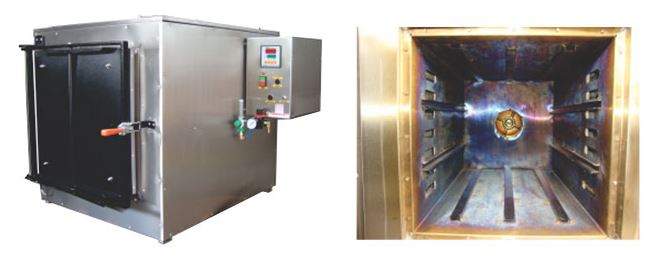
\includegraphics[keepaspectratio=true,scale=0.8]{figuras/forno_mufla.JPG}
	\caption{Imagem ilustrativa de forno para tratamento térmico.}
\end{figure}

\subsubsection{Aplicações}

Fornos de câmara para o recozimento, endurecimento, têmpera e envelhecimento (tratamentos térmicos de metalurgia) com circulação de ar.

\subsubsection{Características}

\begin{itemize}
	\item Sensor de Temperatura;
	\item Isolamento Térmico: em fibra cerâmica pré-moldadas;
	\item Estrutura do Forno: totalmente em aço inoxidável com programador de temperatura digital micro processado com programação de rampas e set-point;
	\item Porta localizada na parte frontal com abertura lateral, para o lado esquerdo;
	\item Painel de controle montado com caixa metálica localizado na lateral do forno, separado do corpo do aquecimento;
	\item Chave geral (disjuntor), sinalizador de painel ligado e programador de tempo e temperatura;
	\item Modelos como capacidade entre 20 e 380 litros, potência de 11 a 35kW e temperatura máxima de até $800 \degree \text{C}$.
\end{itemize}

\subsection{Forno para Laboratório}

\begin{figure}[!h]
	\centering
	\label{forno_laboratorio}
	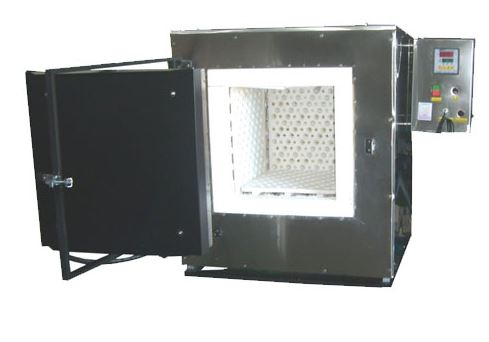
\includegraphics[keepaspectratio=true,scale=0.8]{figuras/forno_laboratorio.JPG}
	\caption{Imagem ilustrativa de Forno para laboratório.}
\end{figure}

\subsubsection{Aplicações}

Forno dedicado à laboratórios de química, cerâmica e metalurgia.

\subsubsection{Características}

\begin{itemize}
	\item Sensor de Temperatura e controlador de temperatura;
	\item Isolamento Térmico: fibra cerâmica pré-moldada e tijolos isolantes superleves;
	\item Controlador de Temperatura;
	\item Estrutura do Forno: Estrutura total em aço inoxidável;
	\item Aquecimento em todas as paredes e porta e sistema de Acionamento de Gás;
	\item Precisão de controle em um ponto de $\pm 5 \degree \text{C}$;
	\item Modelos como capacidade entre 10 e 150 litros, potência de 8 a 18kW e temperatura máxima de até $1320 \degree \text{C}$.
\end{itemize}

\subsection{Forno de Laboratório para Tratamentos Térmicos com gases}

\begin{figure}[!h]
	\centering
	\label{forno_gases}
	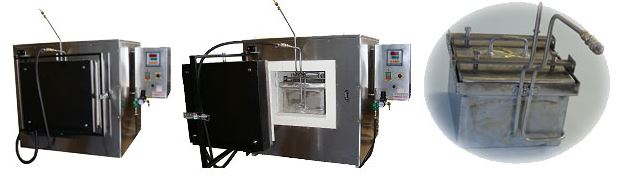
\includegraphics[keepaspectratio=true,scale=0.8]{figuras/forno_gases.JPG}
	\caption{Imagem ilustrativa de Forno de laboratório.}
\end{figure}

\subsubsection{Aplicações}

Forno dedicado à tratamentos térmicos de metalurgia com caixa de gases.

\subsubsection{Características}

\begin{itemize}
	\item Caixa de aço inox para tratamento térmico com injeção de gás regulável para tratamentos especiais para todos os tipos de gases;
	\item Isolação térmica de fibra cerâmica pré - moldada e tijolos isolantes super leves;
	\item Estrutura total em aço inoxidável;
	\item Aquecimento em todas as paredes e porta para os fornos de 20 ou mais litros;
	\item Uniforme distribuição de temperatura;
	\item Controlador micro processado, PID, 10 rampas e 10 patamares;
	\item Termopar tipo “S”;
	\item Controle de segurança para excesso de temperatura e quebra de termopar;
	\item Opcional - Comunicação com o microcomputador, mais software gráfico;
	\item Modelos como capacidade entre 40 e 60 litros, potência de 14 a 16kW e temperatura máxima de até $1280 \degree \text{C}$.
\end{itemize}

\section{Requisitos}

\subsection{Requisitos Operacionais}

\begin{itemize}
	\item A temperatura interna do forno será de até $1200 \degree \text{C}$;
	\item Temperatura externa máxima de $60 \degree \text{C}$;
	\item Obter dados do aquecimento;
	\item Tratamento térmico para aços;
	\item Materiais de pequeno porte;
	\item Cadastro de Usuários;
	\item Seletor de Temperatura;
	\item Iniciar Processo de Tratamento;
	\item Histórico de Sessão;
	\item Sistema de Segurança;
	\item Informações sobre os Processos;
	\item Sistema de Login;
	\item Variação da temperatura de aquecimento controlada.
\end{itemize}

\subsection{Requisitos Técnicos}

\begin{itemize}
	\item Potencia fornecida de 3 KW;
	\item NR – 6;
	\item NR – 10;
	\item NR – 12;
	\item NR – 14;
	\item NR – 15;
	\item Valor das resistencias;
	\item Tijolos Refratários;
	\item Tijolos Refratários;
	\item Dimensionamento interno do forno;
	\item Isolamento com uma manta térmica;
	\item Limite das dimensõe do aço que pode ser tratado no forno;
	\item Sistema de alimentação do forno por eletricidade;
	\item Sensor Termopar tipo K;
	\item Raspberry Pi 2;
	\item Circuito de condicionamento de sinal;
	\item Circuito de controle on/off;
	\item Django Framework;
	\item REST Framework;
	\item Linguagem de Programação Python;
	\item ReactJS.
\end{itemize}

\section{Objetivo Geral}

Projetar e construir um forno de tratamento térmico para experimentos acadêmicos.

\subsection{Objetivos Específicos}

\begin{itemize}
	\item Temperatura do forno até $1200 \degree \text{C}$ com controle liga desliga;
	\item Camada externa com temperatura de até $60 \degree \text{C}$ segundo recomendação da OSHA (Opacional Safety and Health Administration – orgão americano de segurança do trabalhador);
	\item Variação da temperatura de $\pm 20 \degree \text{C}$;
	\item Interface web responsível para controle remoto e relatórios;
	\item Sistema de segurança.

\end{itemize}
